\documentclass[11pt]{scrartcl}
\usepackage[T1]{fontenc}
\usepackage[utf8]{inputenc}

\title{Computer Systems Week 5 Lab}
\author{Daniel Coady (102084174)}
\date{10/09/2019}

\usepackage{graphicx}

\begin{document}

\maketitle

\section*{Assignment Planning}
\subsection*{Component Requirements}
For this assignment, I believe that the following components will be required for
the following stages:

\bigskip

\begin{tabular}{p{2cm} p{10cm}}
    Stage one & This should only require a JK flip flop with connections that allow
                for turning on the circuit and toggling it \\[1em]
    Stage two & For this stage a simple stack circuit should suffice for both storing
                and displaying the state of the volume \\[1em]
    Stage three & Two bi-directional mod 10 counters should allow for the storing
                  of values to display on two hex displays \\[1em]
    Stage four & This might be tough to implement, but using and gates to control
                 whether we allow signal through to the outputs may be the best
                 solution. This said, it might not be the best or most elegant
                 solution.\\[1em]
    Stage five & In theory, this should be fairly trivial. Using simple registers
                 for each of the individual circuits should allow for us to store the
                 state of all the components. When restoring, there will need to be
                 some logic that allows for the instant setting of states, which
                 may be difficult depending on how previous stages have been completed \\[1em]
\end{tabular}

\pagebreak

As well as the above components, I feel that a simple latch for buttons would be
helpful for some circuits where holding a button is not a reasonable way to give
inputs to a circuit.

\begin{figure}[h]
    \centering
    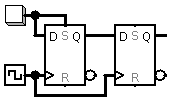
\includegraphics{images/buttonlatch.png}
    \caption{A simple latch for a button to remember the state for the next clock cycle}
\end{figure}

\begin{figure}[h]
    \centering
    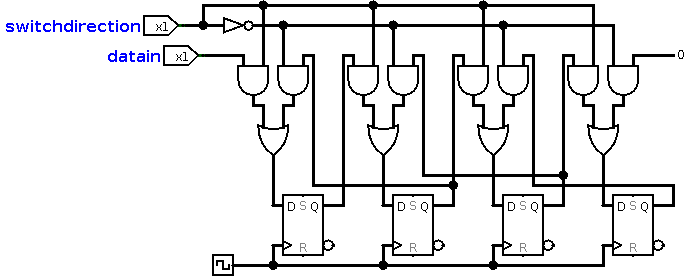
\includegraphics[scale=0.5]{images/stack.png}
    \caption{A stack that can be used for the volume control circuit}
\end{figure}

\begin{figure}[h]
    \centering
    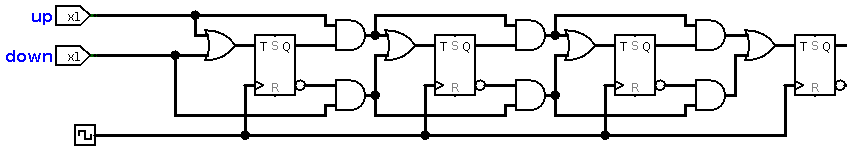
\includegraphics[scale=0.4]{images/counter.png}
    \caption{A bi-directional counter that can form the basis of our track counter system}
\end{figure}

\end{document}
